\chapter{A Basic Artificial Neural Network}

\section{Basic Artificial Neural Network}
%This model is just a model for a class of parameterized function with some special function structure which can be presented simply using some simple network graph.
This method is began from the approximation of neural network in human.
\subsection{basic element: Nonlinear active function with affine map}
M-P element(approximation of one neuron): this is a very simple example for interpolating a function $f: \mathbb{R}^m \to \mathbb{R}$, with the next definition:
\begin{equation}\label{eq:M-P}
f_{M-P}(x) = \sigma( w \cdot x + b)
\end{equation}
with $w  \in \mathbb{R}^{m} \}$ and $g$ is called active function which can be chosen like:
\begin{equation}
\sigma (x) = \frac{1}{1 + e^{-x}},
\end{equation}
or
\begin{equation}
\sigma(x) = tanh(x) = \frac{e^x - e^{-x}}{e^x + e^{-x}}.
\end{equation}
Basically, this two functions both smooth and have two horizontal asymptotic lines, which can be seen as a smoothing approximation for
\begin{equation}
H(x) =
\begin{cases}
1  &\text{if}  ~x < 0, \\
0 &\text{if}~ x \le 0.
\end{cases}
\end{equation}
But now, the most commonly used activation function is the so-called ``Rectified Linear Unit'' (ReLU), which is defined by
\begin{equation}
{\rm ReLU}(x) = \max\{0,x\}.
\end{equation}
We will talk about some basic stuff about variant of activation function in the next chapter and it is also very important in the approximation theory for such as one hidden layer ANN networks.
This is often shown as the next picture:
\begin{figure}[!ht]
	\center{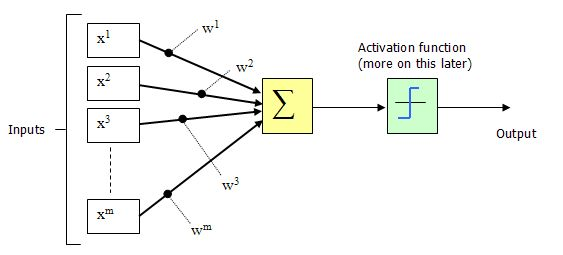
\includegraphics[width=10cm] {M-P.jpeg}}
	\caption{ANN}
\end{figure}

\subsection{neural network}
Now we want to use this simple basic element to construct some more complex model(from one neuron to neural network). A bionic but simple construction is to increase the basic element in both horizontal and vertical direction, which means the network would be like:
\begin{figure}[!ht]
	\center{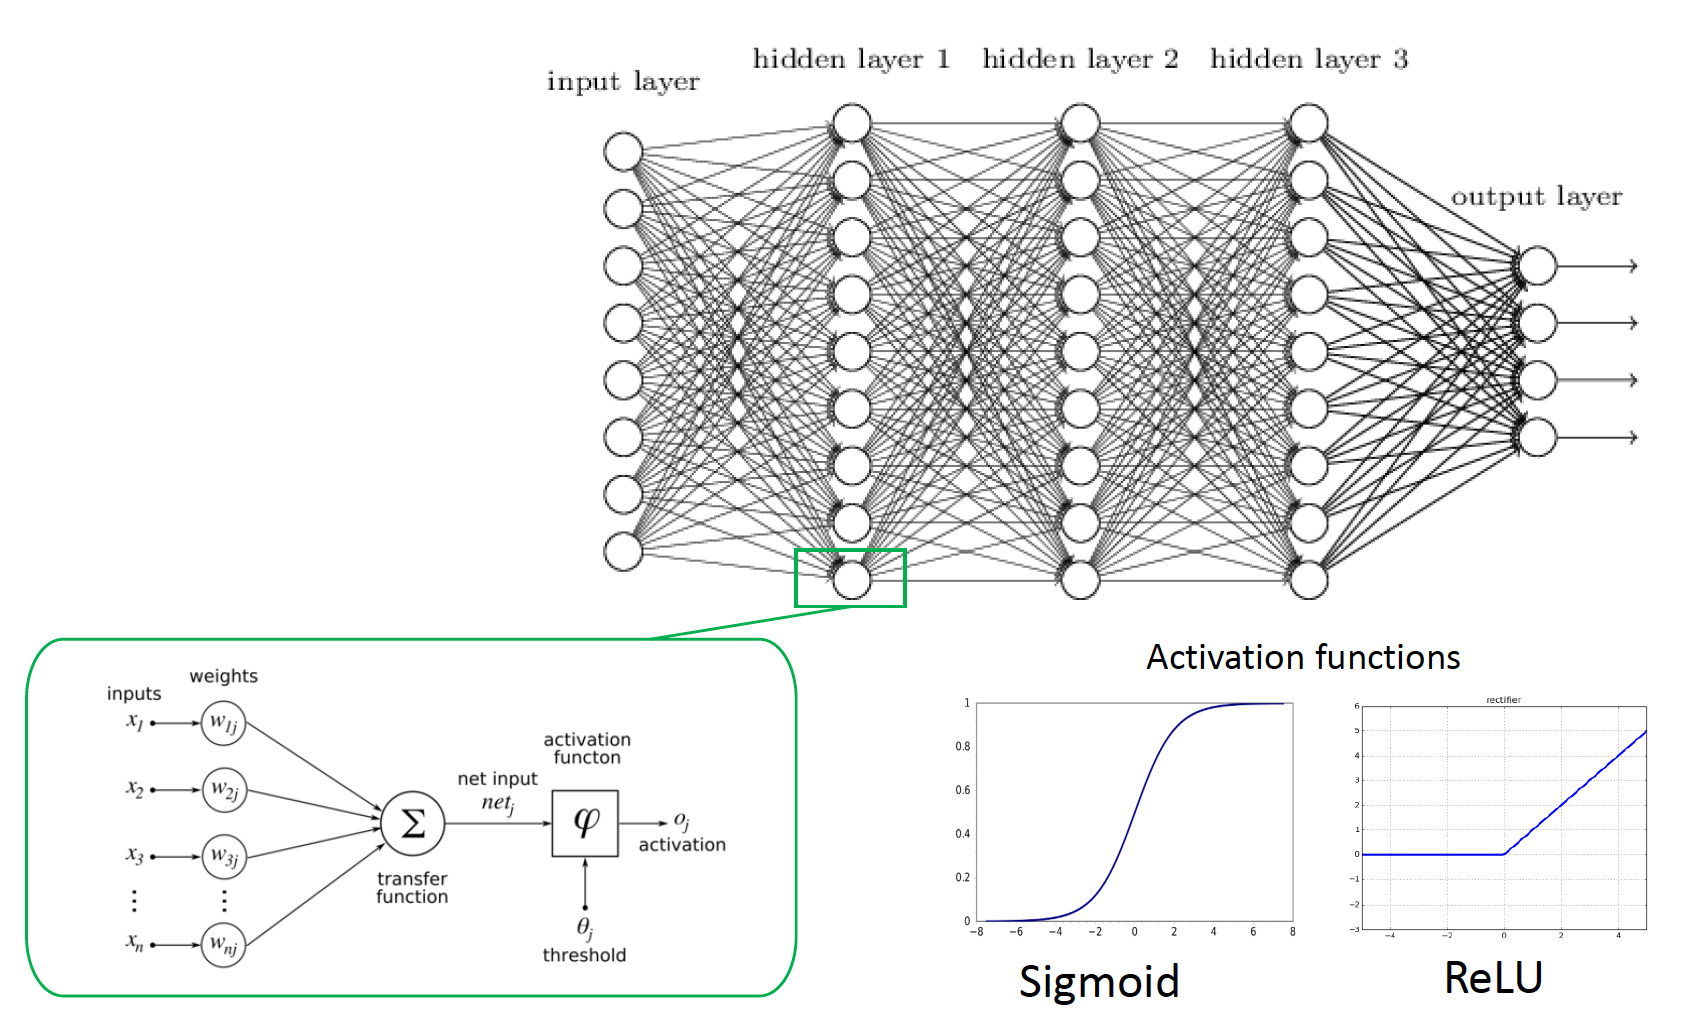
\includegraphics[width=12cm,height=6cm] {ANN.png}}
	\caption{ANN}
\end{figure}

This is called fully connected feedforward neural network. Now we want to give a more compressive expression, we collect all the output in $k$-th level $[f^{k}]_l$ $l = 1,\cdots, n_k$.
So we can have the output in $k+1$-th level under this setting with
\begin{equation}
{f}^{k+1} = \theta^{k+1}\circ \sigma (f^{k})
\end{equation}
with
\begin{equation}
\theta^k(x) = w^kx+b \in\mathbb{R}^{n_{k+1}},
\end{equation} 
where 
\begin{equation}
w^k= 
\begin{pmatrix}
w_1 \\
\vdots \\
w_{n_{k+1}}
\end{pmatrix}
\end{equation}
with $w_i \in \mathbb{R}^{n_k}$.

So, we get the final iterative definition with the last output and initial input of this network like:
\begin{equation}
\begin{cases}
f^{0} &= \theta^0(x), \\
f^{\ell} &= \theta^{\ell}\circ \sigma(f^{\ell-1}), \quad \ell = 1:J, \\
f(x;\Theta) &= f^J.
\end{cases}
\end{equation}
Here we note 
\begin{equation}
\Theta = \{ (\theta^0, \cdots, \theta^J) \}.
\end{equation}

%\subsection{Interpolation by optimization}
%So the  interpolation process can be seen as a optimization problem in the special function class if the activation function for every elements and  the network structure parameter $\mathcal{N}_K$ are given:
%\begin{equation}
%\mathcal{F} = \{\bm{f}_K(W_K;\bm{x}) ~|~  \bm{f}_0 = (\bm{x}^{T},1)^{T}\},
%\end{equation}
%and the optimization problem can be seen as
%\begin{equation}
%%\mathop{\min}_{f \in \mathcal{F}}  \frac{1}{N}\sum_{i=1}^N \|f(X^i) - Y^i\|^2 =
%\mathop{\min}_{W_K \in T_3(\mathcal{N}_K)}  L(W_K) := \frac{1}{N}\sum_{i=1}^N \|\bm{f}_K(W_K; X^i) - Y^i\|^2.
%\end{equation}
%But $\mathcal{F}$ this is neither a linear space nor a convex set.

%\iffalse
\section{Back-Propagation}
Here we will talk about how to compute $\nabla_{\Theta} f(x;\Theta)$ by using chain rule which is called BP algorithm in deep learning. 
Thus we have
\begin{equation}
\frac{\partial {f}(x; \Theta)}{ \partial w^k} = \frac{\partial {f}^J}{\partial {f}^{J-1}} \cdot \frac{ \partial {f}_{J-1}}{\partial {f}^{J-2}} \cdots \frac{ \partial {f}^k}{\partial w^k}.
\end{equation}
We can see from the above that, we only need to compute those terms like:
\begin{equation}
 \frac{ \partial {f}^k}{\partial w^{k}}  \quad \text{and} \quad \frac{\partial {f}^k}{\partial {f}^{k-1}}  \quad k = 1,2,\cdots,J.
\end{equation}


We have
\begin{equation}\label{eq:partial-f}
 \frac{\partial {f}^k}{\partial {f}^{k-1}} =
w^k{\rm Diag}(\sigma'(f^{k-1})) ,
\end{equation}
and
\begin{equation}
\frac{ \partial {f}^k}{\partial w^{k}}  = \delta \otimes \sigma(f^{k-1}).
\end{equation}


In short, BP algorithm can be expressed as:
\begin{algorithm}[H]
\begin{algorithmic}[1]
\State {\bf{Input:}}  $X^i$ and $W_K$;
\For{$k = K:-1:1$}
\State Compute and save
$$\frac{ \partial {f}^k}{\partial w^{k}}  \quad \text{and} \quad \frac{\partial {f}^k}{\partial {f}^{k-1}}$$.
\State Compute
    $$\frac{ \partial {f}^J}{\partial w^{k}} = \frac{\partial {f}^J}{\partial {f}^{J-1}} \cdot \frac{ \partial {f}^{J-1}}{\partial {f}^{J-2}} \cdots \frac{ \partial {f}^k}{\partial w^{k}}$$ 
\EndFor
\end{algorithmic}
\caption{Back-Propagation Algorithm}
\end{algorithm}

